\normaltrue \difficilefalse \tdifficilefalse
\correctiontrue

%\UPSTIidClasse{11} % 11 sup, 12 spé
%\renewcommand{\UPSTIidClasse}{12}

\exer{Train simple $\star$ \label{C2:06:23}}
\setcounter{question}{0}\UPSTIcompetence[2]{A3-05}
\UPSTIcompetence[2]{C2-06}
\index{Compétence C2-06}
\index{Train d'engrenages simple}
\ifcorrection
\else
\textbf{Pas de corrigé pour cet exercice.}
\fi

\ifprof
\else
Soit le train d'engrenages suivant. 
\begin{center}
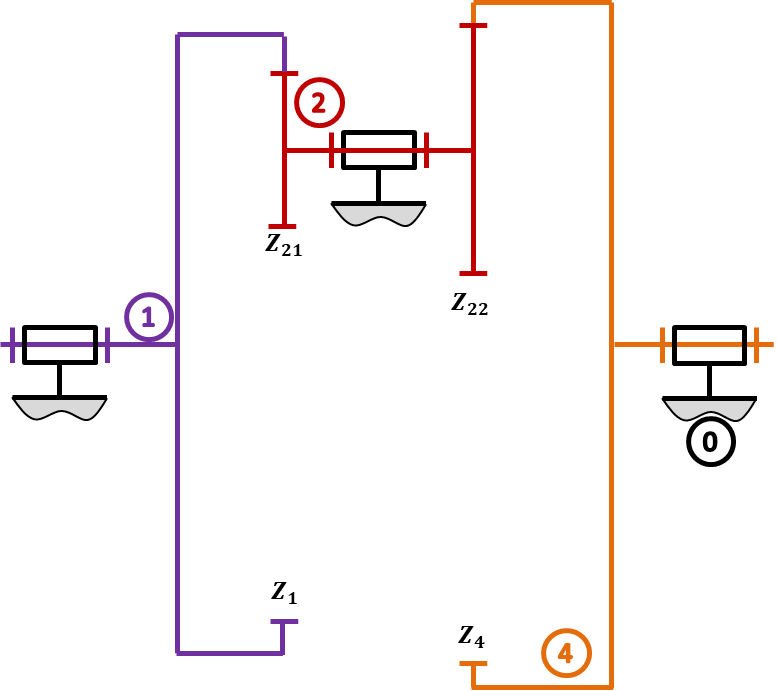
\includegraphics[width=.7\linewidth]{23_01}
\end{center}
\fi


\question{Tracer le graphe des liaisons.}
\ifprof
\else
\fi

\question{Déterminer $\dfrac{\omega_{4/0}}{\omega_{1/0}}$ en fonction du nombre de dents des roues dentées.}
\ifprof ~\\
On a $\dfrac{\omega_{4/0}}{\omega_{1/0}}=\dfrac{Z_1Z_{22}}{Z_4Z_{21}}$.
\else
\fi



\ifprof
\else
\begin{flushright}
\footnotesize{Corrigé  voir \ref{C2:06:23}.}
\end{flushright}%
\fi